This section describes techniques useful in global sensitivity analysis, specifically
\begin{itemize}
\item Polynomial Chaos Expansion (PCE)
\item Sparse regression with application to PCE, including LASSO/Basis Pursuit~(BP) algorithms
%\item $L_1$ aka $\ell_1$-norm regularisation (versus $L_2$, ie. least-squares)
\item Multifidelity Monte-Carlo~(MFMC)
\item Multilevel Monte-Carlo~(MLMC)  and Multi-Index Monte-Carlo~(MIMC)
\end{itemize}
\paragraph{The `curse of dimensionality'}
The need for special techniques arises from the need to treat problems
typically with a large number~$d$ of parameters that give
rise to the so-called  `curse of dimensionality'. The curse defeats
simple uniform sampling strategies where supposing that $10$~samples are taken for
each parameter, the number of samples required is $10^d$.
This fact motivates use of Monte-Carlo~(MC) sampling
which has costs independent of~$d$ but gives rise to a slowly reducing error$\propto 1/\sqrt{N}$ in 
the calculation of averages, where $N$ is the number of samples.

To calculate more accurate statistics, use is made of
Quasi-Monte-Carlo~(QMC) sampling, see the appended \Sec{QMC},
and sparse (quadrature) sampling~\Sec{sparse} which can achieve errors$\propto (\ln N)^d/N$.
Even in this expression, the power-law dependence on~$d$ restricts use of the technique to values of~$d$ of order ten or so,
more precise values depending on the cost of a single sample calculation, hence the need
for techniques of sparse regression to identify a restricted set of parameters.
%for Point~2 above.

\subsubsection{Polynomial Chaos Expansion~(PCE)}\label{sec:PCE}

Polynomial Chaos Expansion~(PCE), also known as the Wiener chaos expansion \cite{Wi38Homo},
is a method for determining the evolution of uncertainty in a dynamical system
where there is imperfect knowledge of the system parameters.
Uncertain parameters and variables are supposed to depend on a normally distributed random variable $\theta$,
and are then expressed using a Hermite expansion.
For example, density $n(\x,t)$, usually a function of position $\x$ and time $t$, would gain an additional $\theta$-dependence and 
be written
\begin{align}
	\label{eq:Hermite_expansion}
	n(\x,t,\theta) = \sum_{j=0}^{N_H} n_j(\x,t)H_j(\theta),
\end{align}
where $n_j(\x,t)$ are deterministic coefficients and $H_j$ are the Hermite polynomials.
Hermite polynomials are used as these are orthogonal with respect to a Gaussian (\emph{i.e.}\ normal distribution) weight,
\begin{align}
	\label{eq:orthogonality}
	\langle H_n | H_m \rangle =
	\frac{1}{2^nn!}\int_{-\infty}^{\infty} H_n(\theta)H_m(\theta)\frac{e^{-\theta^2}}{\sqrt{\pi}} \ \mathrm{d}\theta = \delta_{nm},
\end{align}
where $\delta_{nm}$ is the Kronecker which is 1 if $n=m$ and 0 otherwise.
Statistical properties, which are moments of $n$ with respect to $\theta$, are then known simply in terms of the expansion coefficients.
For example, the expected value of $n$ is
\begin{align}
	\mathbb{E}(n) \equiv \int_{-\infty}^{\infty} n(\x,t,\theta)\ \mathrm{d}\theta = n_0(\x,t).
\end{align}
Moreover, by taking the inner product of the model equations with each Hermite polynomial in turn,
one obtains a set of moment equations for the evolution of the coefficients $n_j$.
For example, taking moments of the equation for the conservation of density,
\begin{align}
	\label{eq:density}
	\pd{n}{t} + \pd{(nu)}{x} = 0,
\end{align}
yields the $N_H+1$ equations
\begin{align}
	\label{eq:moment_hierarchy}
	\pd{n_k}{t} + \sum_{i=0}^{N_H}\sum_{j=0}^{N_H}e_{ijk}\pd{(n_iu_j)}{x} = 0,
\end{align}
with $e_{ijk}\equiv \int_{-\infty}^{\infty}H_iH_jH_k\ \mathrm{d}\theta$ being (easily-computable) integrals.
Equation~\eqref{eq:moment_hierarchy} also appears in the Equations document~\cite{pappeqs}.
Solving~\eqref{eq:moment_hierarchy} allows one to reconstruct $n(\x,t,\theta)$ via \eqref{eq:Hermite_expansion}, which gives the density along with a quantification of its uncertainty through $\theta$. 

This method may be generalised to include a set of random variables $\{\theta_i\}$, in which case an expansion analogous to \eqref{eq:Hermite_expansion} is made using tensor Hermite polynomials.

The Hermite expansion approach is appropriate only for $\theta$ a normally distributed random variable (or certain similar types, like log-normal distributions).
For other distributions, convergence of the expansion \eqref{eq:Hermite_expansion} with $N_H$ can be extremely slow.
However using non-normal distributions is often desirable; for example, it might be known that errors are non-negative, or uniformly distributed.
To allow modelling with non-normal distributions, Xiu \cite{xiu04} introduced Generalised Polynomial Chaos (gPC).
In gPC, the random variable $\theta$ is generalised to be a random variable with any distribution function $f$.
The Hermite polynomial expansion is then replaced with an expansion in the set of orthogonal polynomials whose weight function is $f$.
For example, if $\theta$ is uniformly distributed, the expansion is in Legendre polynomials.
The gPC theory also supports discrete random variables, such as the Poisson and the binomial distributions; 
a list of random variables and their corresponding orthogonal polynomials are given in \cite[Table 2.1]{xiu04}.

The method described above is \emph{intrusive}, that is,
if one only has software to solve the original problem \eqref{eq:density} for $n$,
then non-trivial changes are likely required in order to solve \eqref{eq:moment_hierarchy} for $n_k$.
An alternative non-intrusive approach may be derived as follows.
Suppose the solution is sampled at a set of $N$~random
points~$\{\theta_j\}_{j=1}^{N}$,
and construe $n$ as a distribution in probability space, viz.
\begin{equation} \label{eq:dfnexpn}
n(x,t,\theta) = \sum_{j=0}^{N} n_{sj}(x,t)\delta(\theta-\theta_j).
\end{equation}
Equating \eqref{eq:dfnexpn} with \eqref{eq:Hermite_expansion} in the weak sense, there obtains
\begin{equation} \label{eq:hermweak}
\left\langle\sum_{j=0}^{N} n_{sj}(x,t)\delta(\theta-\theta_j) \Bigg|  H_k(\theta)\right\rangle =
\left\langle\sum_{j=0}^{N_H} n_{j}(x,t) H_j (\theta) \Bigg| H_k(\theta)\right\rangle,
\end{equation}
where $\langle\cdot|\cdot \rangle$ is the inner product defined in \eqref{eq:orthogonality}, so that
\begin{equation} \label{eq:hermres}
n_k(x,t) = \frac{1}{2^kk!\sqrt{\pi}}\sum_{j=0}^{N_H} n_{sj}(x,t)H_k(\theta_j) e^{-\theta_j^2}.
\end{equation}
This expression for $n_k$ may be calculated using only knowledge of $n$ from solving the original equation \eqref{eq:density}.

\subsubsection{Sparse linear regression}\label{sec:sparsereg}

\paragraph{Linear regression}
Suppose a data set $\{y_i,x_{1i},\ldots,x_{di}\}_{i=1}^{N}$ to consist of
$N$ observations of the dependent variable $y$ and the $d$ independent
variables $\x$,
supposed related by the model $y=\x\boldsymbol{\beta}$,
where $\boldsymbol{\beta}^T=(\beta_1,\ldots,\beta_d)$ is a vector of unknown coefficients of the model.
The classical linear regression problem determines $\boldsymbol{\beta}$ by minimising the $L_2$-norm error,
\begin{align}
	\label{eq:linear_regression}
\min_{\boldsymbol{\beta}\in \mathbb{R}^d}\|y - \x\boldsymbol{\beta}\|^2.
\end{align}
When there are more observations than parameters, $N>d$, this has the
well-defined solution $\boldsymbol{\beta}^*=(\x^T\x)^{-1}\x^Ty$.

\paragraph{Sparse linear regression}
In some applications there are many more observations than parameters $N\gg d$,
and moreover many of the observation points $x_j$ may be expected to be irrelevant for
determining $y$.
In this case, many of the coefficients $\beta_i$ would be expected to be zero,
but it will not known \emph{a priori} which can be neglected.
Many approaches have been developed to incorporate sparsity into linear regression.
This section focusses on 
\begin{itemize}
\item Sequential Least-Squares' Thresholding~(SLSQT)
\item Best Subset Selection %Forwards Stepwise Regression,
\item Ridge Regression
\item LASSO
\end{itemize}
The last three of these
may all be formulated as regularised least-squares optimisation,
\emph{i.e.}\ least-squares subject to an additional inequality constraint.
%and Basis Pursuit.
For simplicity, the following discussion is restricted to the case
when the independent variables $\x_i$ are orthonormal,
$\langle\x_i | \x_j\rangle = \delta_{ij}$,
which applies when the independent variables are the basis functions from a
polynomial chaos expansion.

\paragraph{Sequential Least-Squares' Thresholding~(SLSQT)} is simply described 
as a sequence of least-squares' fits in which after each fit
regression coefficients that drop below some researcher-fixed threshold are set and
remain zero thereafter.
This has proved very successful for Brunton~et~al~\cite{Br16Disc}.

\paragraph{Best subset selection}
A natural formulation for seeking a sparse coefficient vector $\boldsymbol{\beta}$
is to restrict $\boldsymbol{\beta}$ to having a small number of non-zero entries.
The linear regression problem \eqref{eq:linear_regression} is modified to 
\begin{align}
	\label{eq:best_subset}
\min_{\boldsymbol{\beta}\in \mathbb{R}^d}\|y - \x\boldsymbol{\beta}\|^2_2
	\hspace{0.5cm}
	\mathrm{subject\ to}
	\hspace{0.5cm}
	\|\boldsymbol{\beta}\|_0 \leq C.
\end{align}
where $\|\boldsymbol{\beta}\|_0$ is the ``0-norm'' which simply counts the number of non-zero elements of $\boldsymbol{\beta}$.
This is known as ``Best Subset Selection''
as the constraint on $\bbeta$ restricts the nonzero coefficients to a $k$-dimensional subspace of the original problem.

Equation \eqref{eq:best_subset} may be written in Lagrangian form,
\begin{align}
	\label{eq:best_subset_lagrangian_form}
	\min_{\boldsymbol{\beta}\in \mathbb{R}^d}\left( \frac{1}{N}\|y - \x\boldsymbol{\beta}\|^2_2 + \lambda \|\boldsymbol{\beta}\|_0 \right),
\end{align}
which is solved by 
\begin{align}
	\beta_j 
	= \mathcal{H}_{\sqrt{N\lambda}}(\beta^*_j) 
	= \beta^*_j \mathcal{I}\left(|\beta_j^*|>\sqrt{N\lambda}\right)
\end{align}
where $\mathcal{I}$ is the indicator function that is unity if its argument is true, and zero otherwise, and $\bbeta^*=(\x^T\x)^{-1}\x^T\bbeta$ is the solution to the ordinary least-squares problem.
Here $\mathcal{H}_{\alpha}$ is the ``hard thresholding function'', which sets
coefficients to zero once they are sufficiently small, but leaves other
coefficients untouched.

This approach is however computationally infeasible. 
%Even if p is used elsewhere, we should really call this the p-norm. 'p-norm' is more of a proper noun than a use of p as notation. 
This is because the ``0-norm'', the $p\to0$ limit of the $p$-norm, $\|\boldsymbol{\beta}\|_p=\left(\sum_i \beta_i^p\right)^{1/p}$,
is not actually a norm (as, for example, $\|2\boldsymbol{\beta}\|_0\neq 2\|\boldsymbol{\beta}\|_0$).
This means one cannot minimise $\|\cdot\|_0$ except by exhaustive search.
Therefore other methods replace the ``0-norm'' with $p$-norms that are computationally tractable.


\hyphenation{co-dependencies}
\paragraph{Ridge regression} 
In ridge regression, also known as $L_2$ regularisation, the ``0-norm'' is replaced with the Euclidean 2-norm,
\begin{align}
	\label{eq:ridge_regression}
	\min_{\boldsymbol{\beta}\in \mathbb{R}^d}\left( \frac{1}{N}\|y - \x\boldsymbol{\beta}\|^2_2 + \lambda \|\boldsymbol{\beta}\|_2^2 \right),
\end{align}
This approach, a variant of Tikhonov regularisation, mitigates the problems due to dependencies
among the variables~$x_i$.
As $\nabla\|\x\|^2_2= -\x/\|\x\|^2_2$ is invariant under a rescaling of~$\x$, 
\Eq{ridge_regression} has the solution
\begin{align}
	\label{eq:ridge_regression_solution}
	\beta_j 
	= (1+N\lambda)^{-1} \beta^*_j.
\end{align}
%This method is a small modification to the ordinary least-squares problem
%and is therefore tractable.
%It also suitable for problems with large numbers of parameters
%because it mitigates the problem of multicollinearity.
%Multicollinearity is where the ``independent'' variables $x_i$ 
%actually contain codependencies,
%which in computation leads to the values of $\bbeta$ being unreliable
%or unstable.
%Ridge regression reduces the variance of the $\bbeta$ values,
%reducing the effect of codependencies.
%
Evidently, this solution %\eqref{eq:ridge_regression_solution}
does not increase the sparsity of the solution
and so does not reduce the number of model parameters, leading to consideration
of use of the 1-norm in \Eq{ridge_regression}. %so it may be used in
%conjunction with a method that does, as follows.

\paragraph{LASSO}
The LASSO method, also called basis pursuit denoising, $L_1$ regularisation, or
`compressed sensing'~(CS),
turns out to yield the favourable features of
Best Subset Selection and Ridge Regression.
In LASSO, the ``0-norm'' is replaced with the 1-norm, $\|\boldsymbol{\beta}\|_1=\sum_i |\beta_i|$, in equation \eqref{eq:best_subset},
\begin{align}
	\label{eq:lasso}
	\min_{\boldsymbol{\beta}\in \mathbb{R}^d}\left( \frac{1}{N}\|y - \x\boldsymbol{\beta}\|^2_2 + \lambda \|\boldsymbol{\beta}\|_1 \right).
\end{align}
Although not obvious, it may be shown using the Karush-Kuhn-Tucker conditions for constrained optimisation
that the 1-norm is also minimised by values of $\boldsymbol{\beta}$ containing exact zeros;
moreover, smaller values of~$C$ in \eqref{eq:best_subset} yields $\boldsymbol{\beta}$ with more zeros.
The 1-norm, being a norm, is also computationally tractable.

The solution to \eqref{eq:lasso} is
\begin{align}
	\label{eq:lasso_solution}
	\beta_j 
	= \mathcal{S}_{n\lambda}\left(\beta_j^*\right)
	= \beta_j^* \max\left( 0, 1 - \frac{N\lambda}{|\beta_j^*|}\right),
\end{align}
where $\mathcal{S}_{\alpha}$ is the ``soft thresholding function''.
This solution both shifts coefficient values towards zero,
and sets the smaller values to zero, increasing the sparsity.

\subsubsection{Multifidelity Monte-Carlo}\label{sec:mfmc}

\paragraph{Multifidelity modelling}
In conventional modelling, normally a ``high-fidelity'' model is produced which captures
as faithfully as possible the system being modelled.  
%We may think of this model as a function $\fone$ that maps input values $z$ to
%output values $y$.
Such models can be computationally expensive,
motivating the use of low-fidelity, or reduced, models
which approximate the same system but that, for example,
describe simplified physics, or use a lower resolution grid.
Reduced models are much cheaper,
but may be much less able to predict the behaviour of a physical system.
Moreover it may be difficult to certify the
model by quantifying uncertainties.

Multifidelity modelling is an approach between these two extremes.
It uses both high-fidelity and (possibly multiple) low-fidelity models
in an attempt to place guarantees on the properties of the solution.

\paragraph{Monte-Carlo sampling}
In Monte-Carlo sampling, there is an uncertain input (random variable $Z$) to a high-fidelity model, $\fone$.
The outputs from the model $\fone(Z)$ are also uncertain,
so the goal is to calculate statistics,
such as the expected value of the output, $s=\mathbb{E}(\fone(Z))$.
Estimators for this statistic are made by making $N$ evaluations of the model,
that is, taking $N$ realisations $z_i$ from $Z$ and computing
\begin{align}
	\label{eq:MCestimator}
\hat{s}=\bar{y}^{(1)}_N = \frac{1}{N}\sum_{i=1}^N\fone(z_i).
\end{align}
If the work of evaluating the model once is $W_1$, then the Monte-Carlo process costs $NW_1$ work.

\paragraph{Multifidelity Monte-Carlo (MFMC)}
In multifidelity Monte-Carlo, the single high-fidelity model $\fone$ supplemented with a collection of $K-1$ lower-fidelity ``surrogate'' models,
$\ftwo$, \ldots, $\fK$,
where fidelity decreases with increasing index.
Model $i$ is evaluated $n_i$ times, where higher fidelity models are evaluated fewer times, $n_1 \leq n_2 \leq \ldots \leq n_K$.
Define mean estimators $\bar{y}^{(j)}_{n} = \frac{1}{n}\sum_{i=1}^n f^{(j)}(z_i)$ (from calling
the~$j$th model $n$~times),
and from these construct the MFMC estimator for $s$,
\begin{align}
	\label{eq:MFMCestimator}
	\hat{s} = \bar{y}^{(1)}_{n_1} + \sum_{i=2}^{K}\alpha_i\left(\bar{y}^{(i)}_{n_i} - \bar{y}^{(i)}_{n_{i-1}} \right).
\end{align}
Compared to \eqref{eq:MCestimator}, this requires many fewer evaluations of the high-fidelity model ($n_1\ll N$),
but additional evaluations of the surrogate models.
In \eqref{eq:MFMCestimator}, the bracketed term expresses the change in mean estimator of $\bar{y}^{(i)}$ that results from calling model $i$ more times relative to model $i-1$, the model that is one-level higher-fidelity.
The estimator is unbiased,
and moreover gives the freedom to choose the model evaluations $n_1$, $n_2$, $\ldots$, $n_K$
and the coefficients $\alpha_2$, \ldots, $\alpha_K$.

The cost of evaluating $\hat{s}$ is $\sum_{i=1}^{K} W_in_i$.
Because surrogate models are cheaper to compute ($W_1>W_i$ for all $i>1$)
and many fewer evaluations of the high-fidelity model ($n_1\ll n$) are anticipated,
this cost is significantly less than the cost $NW_1$ of the conventional Monte-Carlo calculation.
Peherstorfer \emph{et al.} \cite{Pe16Opti} used this approach to obtain the same accuracy as a high-fidelity MC simulation, but with a reduction in runtime of four orders of magnitude.


\paragraph{Multi-Level Monte-Carlo (MLMC)}\label{sec:mlmc}
%MFMA - see Slide 7 of Sa18Spar-ppt
Multi-level Monte-Carlo~(MLMC) is a more efficient way of estimating averages
and other statistics than by means of random or Monte-Carlo~(MC) sampling. 
MLMC is usually associated with the name of Mike~Giles~\cite{Gi16Mult}.
Suppose that a model or surrogate problem may be solved with a range of
spatial and/or temporal resolutions. The basic idea is that sample solutions
computed with different levels of resolution may be combined to produce means
and other statistics 
(giving estimates of uncertainty) as accurately as though all solutions had been
obtained using the finest level.

In more detail, for the example of a steady solution obtained with
different spatial levels of resolution~\cite{Mi13Mult}, the MLMC algorithm is
\begin{enumerate}
\item Construct a hierarchy of meshes, spacings~$h_l$, where $l=0$ is the coarsest level
and $l=L$ is the finest.
\item For each~$l$, draw a level-dependent number~$N_l$ of samples from the parameters/fields
to be sampled, eg.\ 
${\mathbf U}$ denoting a single solution depending on $d$~spatial variables alone.
\item Solve the model or surrogate problem $N_l$ times at each level, giving an
ensemble of solutions~${\mathbf U}^k_l,\;k=1,\ldots N_l$,
\item Estimate the mean (other moments of the distribution follow similarly) as
\begin{equation}\label{eq:telescope}
{\mathbb E}^L[{\mathbf U}]= \sum_{l=0}^L {\mathbb E}_l[{\mathbf U}_l-{\mathbf U}_{l-1}]
\end{equation}
using simple averages~${\mathbb E}_l$ with ${\mathbf U}_{-1}={\mathbf 0}$
\end{enumerate}

Large gains occur when
$N_l=N_0 4^{lp}$ where the solution scheme is of order~$p\leq(d+1)/2$.
A refinement of MLMC, referred to as Multi-Index Monte-Carlo~(MIMC)~\cite{Ha18Mult}
allows for $h_l$ to be different by factors of~$2$ in  different coordinate directions.
As illustrated in \Fig{mimc},
the differences of function values in \Eq{telescope} on two isotropic meshes may be replaced by
differences between values on several different anisotropic meshes.
\begin{figure}[hbtp]
\centerline{\rotatebox{0}{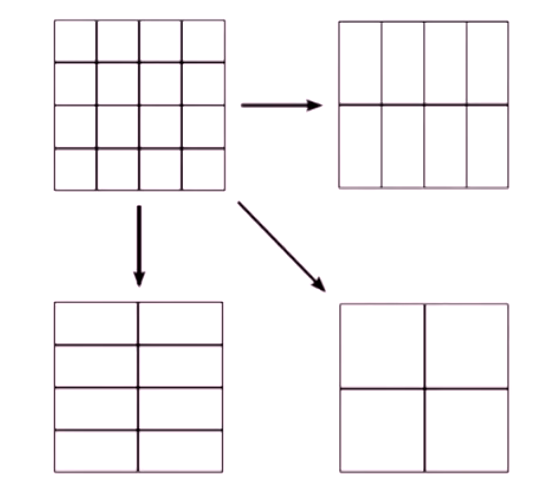
\includegraphics[width=6.5cm]{../png/mimc}}}
\caption{Different meshes for use in MLMC and MIMC in 2-D. In MLMC, only the
bottom right and top left would be differenced in the \protect\Eq{telescope},
whereas all four might be differenced in MIMC, depending on choice of `index set'.
\label{fig:mimc}}
\end{figure}


Note that Najm~\emph{et al}'s work~\cite{Ge19Prog} often focusses on quantities of interest (QoIs)~$Q$ rather
than the whole solution. They also point out that the error in the 
standard deviation is not available in closed form and its calculation 
involves a complicated approximation which they describe~\cite[\S\,III.B.1]{Ge19Prog}.  

%The MLMC estimator of the expectation value of $Q_L$  - the QoI evaluated at the finest resolution 
%level - and its variance can be expanded as
%
%\begin{eqnarray}
%\mathbb{E}(Q_L) \approx \hat{Q}^{ML}_L &=& \sum_{l=0}^L \frac{1}{N_l} \sum_{i=1}^{N_l} \left ( 
%Q_l^{(i)}-Q_{l-1}^{i} \right ) = \sum_{l=0}^L \hat{Y}_l\\
%\mathrm{Var}[\hat{Q}^{ML}_L] &=& \sum_{l=0}^L \frac{1}{N_l} \mathrm{Var}[Y_l].
%\end{eqnarray}
%
%Here $Y_l$ is the difference function between two successive levels and $\hat{Y}_l$ its estimator 
%at the $l$th level.  
%The utility of the MLMC is that, if it is reasonable to assume that $\mathrm{Var}[Y_L] \rightarrow 
%0$ as $l \rightarrow 0$, then the number of samples $N_l$ at each level decreases for increasing 
%$l$.  
%The standard error in the mean can be obtained as the square root of $\mathrm{Var}[\hat{Q}_L^{ML}]$ 
%because the distribution of the MLMC estimator approaches a Gaussian for a large sample size; the 
